\immediate\write18{tex spath3.dtx}
\documentclass{ltxdoc}
\usepackage[T1]{fontenc}
\usepackage{trace}
\usepackage{lmodern}
\usepackage{morefloats}
\usepackage{tikz}
\usetikzlibrary{knots}
\usepackage[numbered]{hypdoc}
\definecolor{lstbgcolor}{rgb}{0.9,0.9,0.9} 
 
\usepackage{listings}
\lstloadlanguages{[LaTeX]TeX}
\lstset{breakatwhitespace=true,breaklines=true,language=TeX}
 
\usepackage{fancyvrb}

\newenvironment{example}
  {\VerbatimEnvironment
   \begin{VerbatimOut}{example.out}}
  {\end{VerbatimOut}
   \begin{center}
   \setlength{\parindent}{0pt}
   \fbox{\begin{minipage}{.9\linewidth}
     \lstset{breakatwhitespace=true,breaklines=true,language=TeX,basicstyle=\small}
     \lstinputlisting[]{example.out}
   \end{minipage}}

   \fbox{\begin{minipage}{.9\linewidth}
     \centering
     \input{example.out}
   \end{minipage}}
\end{center}
}

\providecommand*{\url}{\texttt}
\GetFileInfo{spath3.sty}

\title{Cubes}
\author{Adam Howard}
\date{\today}

\begin{document}
\newcommand{\Depth}{4}
\newcommand{\Height}{4}
\newcommand{\Width}{4}
\maketitle

% (1, 2, 0) with m = 0
\begin{tikzpicture}

\node (w) at (0,5, 0) [minimum width=100pt,minimum height=20pt,thick] {$(1, 2, 0); m = 0$};
\node (x) at (2,0,4.7) [minimum width=100pt,minimum height=20pt,thick] {$S^{1}_{spin}$};
\node (y) at (4. 5,0,2)  [minimum width=100pt,minimum height=20pt,thick] {$K$};
\node (z) at (4.5,2,0)  [minimum width=100pt,minimum height=20pt,thick] {$S^{1}_{bun}$};
\coordinate (O) at (0,0,0);
\coordinate (A) at (0,\Width,0);
\coordinate (B) at (0,\Width,\Height);
\coordinate (C) at (0,0,\Height);
\coordinate (D) at (\Depth,0,0);
\coordinate (E) at (\Depth,\Width,0);
\coordinate (F) at (\Depth,\Width,\Height);  
\coordinate (G) at (\Depth,0,\Height);



\coordinate (W) at (0,\Width/2,0);
\coordinate(X) at (\Depth,\Width/2,0);
\coordinate (Y) at (0,\Width/2,\Height);
\coordinate(Z) at (\Depth,\Width/2,\Height);

\draw[fill=yellow!80,fill opacity=0.3] (C) -- (W) -- (X) -- (G) -- cycle;
\draw[fill=yellow!80,fill opacity=0.3] (Y) -- (A) -- (E) -- (Z) -- cycle;

\draw[green] (W) -- (X);
\draw[green] (Y) -- (Z);

\draw[red, thick] (C) -- (G); %Bottom Back
\draw[red] (O) -- (D); %Bottom Front
\draw[red] (B) -- (F); % Top Front
\draw[red] (A) -- (E); %Top Back

\draw[blue] (C) -- (O); %Bottom Left
\draw[blue] (G) -- (D); %Bottom Right
\draw[blue] (B) -- (A); %Top Left
\draw[blue] (F) -- (E); %Top Right

\draw[black] (C) -- (B); %Front Left
\draw[black] (O) -- (A); %Back Left
\draw[black] (G) -- (F); %Front Right
\draw[black] (D) -- (E); %Back Right

%% Following is for debugging purposes so you can see where the points are
%% These are last so that they show up on top
%\foreach \xy in {O, A, B, C, D, E, F, G, W, X, Y, Z}{
%\node at (\xy) {\xy};
%}
\end{tikzpicture}

%% (1, 2, 0) with m = 1
%This is a much less pleasant cube
\begin{tikzpicture}

%\node (A) at (2,0,2) [minimum width=100pt,minimum height=20pt,thick] {$\mathcal{T}$};
%\node (S) at (4.5,2,0)  [minimum width=100pt,minimum height=20pt,thick] {$S^{1}$};
\node (w) at (0,5, 0) [minimum width=100pt,minimum height=20pt,thick] {$(1, 2, 0); m = 1$};
\node (x) at (2,0,4.7) [minimum width=100pt,minimum height=20pt,thick] {$S^{1}_{spin}$};
\node (y) at (4. 5,0,2)  [minimum width=100pt,minimum height=20pt,thick] {$K$};
\node (z) at (4.5,2,0)  [minimum width=100pt,minimum height=20pt,thick] {$S^{1}_{bun}$};

\coordinate (O) at (0,0,0);
\coordinate (A) at (0,\Width,0);
\coordinate (B) at (0,\Width,\Height);
\coordinate (C) at (0,0,\Height);
\coordinate (D) at (\Depth,0,0);
\coordinate (E) at (\Depth,\Width,0);
\coordinate (F) at (\Depth,\Width,\Height);
\coordinate (G) at (\Depth,0,\Height);



\coordinate (W) at (0,\Width/2,0);
\coordinate(X) at (\Depth,\Width/2,0);
\coordinate (Y) at (0,\Width/2,\Height);
\coordinate(Z) at (\Depth,\Width/2,\Height);

\coordinate (a) at (\Depth/2,\Width,0);
\coordinate(b) at (\Depth/2,\Width,\Height);
\coordinate (c) at (0,\Width,\Height/2);
\coordinate(d) at (\Depth,\Width,\Height/2);

\coordinate (e) at (\Depth/2,0,0);
\coordinate(f) at (\Depth/2,0,\Height);
\coordinate (g) at (0,0,\Height/2);
\coordinate(h) at (\Depth,0,\Height/2);




\draw[fill=yellow!80,fill opacity=0.3] (C) -- (F) -- (a) -- (W) -- cycle;
\draw[fill=yellow!80,fill opacity=0.3] (O) -- (f) -- (Z) -- (E) -- cycle;
\draw[fill=yellow!80,fill opacity=0.3] (Y) -- (b) -- (A) -- cycle;
\draw[fill=yellow!80,fill opacity=0.3] (e) -- (G) -- (X) -- cycle;




\draw[red, thick] (C) -- (G); %Bottom Back
\draw[red] (O) -- (D); %Bottom Front
\draw[red] (B) -- (F); % Top Front
\draw[red] (A) -- (E); %Top Back

\draw[blue] (C) -- (O); %Bottom Left
\draw[blue] (G) -- (D); %Bottom Right
\draw[blue] (B) -- (A); %Top Left
\draw[blue] (F) -- (E); %Top Right

\draw[black] (C) -- (B); %Front Left
\draw[black] (O) -- (A); %Back Left
\draw[black] (G) -- (F); %Front Right
\draw[black] (D) -- (E); %Back Right

%% Following is for debugging purposes so you can see where the points are
%% These are last so that they show up on top
%\foreach \xy in {O, A, B, C, D, E, F, G, W, X, Y, Z, a, b, c, d, e, f, g, h}{
   % \node at (\xy) {\xy};
%}

\end{tikzpicture}

\hspace{50pt}

% (2, 1, 0)  with m = 0
\begin{tikzpicture}
\node (w) at (0,5, 0) [minimum width=100pt,minimum height=20pt,thick] {$(2, 1, 0); m = 0$};
\node (x) at (2,0,4.7) [minimum width=100pt,minimum height=20pt,thick] {$S^{1}_{spin}$};
\node (y) at (4. 5,0,2)  [minimum width=100pt,minimum height=20pt,thick] {$K$};
\node (z) at (4.5,2,0)  [minimum width=100pt,minimum height=20pt,thick] {$S^{1}_{bun}$};
\coordinate (O) at (0,0,0);
\coordinate (A) at (0,\Width,0);
\coordinate (B) at (0,\Width,\Height);
\coordinate (C) at (0,0,\Height);
\coordinate (D) at (\Depth,0,0);
\coordinate (E) at (\Depth,\Width,0);
\coordinate (F) at (\Depth,\Width,\Height);
\coordinate (G) at (\Depth,0,\Height);



\coordinate (W) at (0,\Width/2,0);
\coordinate(X) at (\Depth,\Width/2,0);
\coordinate (Y) at (0,\Width/2,\Height);
\coordinate(Z) at (\Depth,\Width/2,\Height);

\draw[fill=yellow!80,fill opacity=0.3] (C) -- (Z) -- (X) -- (O) -- cycle;
\draw[fill=yellow!80,fill opacity=0.3] (Y) -- (F) -- (E) -- (W) -- cycle;

\draw[green] (Z) -- (X);
\draw[green] (Y) -- (W);

\draw[red, thick] (C) -- (G); %Bottom Back
\draw[red] (O) -- (D); %Bottom Front
\draw[red] (B) -- (F); % Top Front
\draw[red] (A) -- (E); %Top Back

\draw[blue] (C) -- (O); %Bottom Left
\draw[blue] (G) -- (D); %Bottom Right
\draw[blue] (B) -- (A); %Top Left
\draw[blue] (F) -- (E); %Top Right

\draw[black] (C) -- (B); %Front Left
\draw[black] (O) -- (A); %Back Left
\draw[black] (G) -- (F); %Front Right
\draw[black] (D) -- (E); %Back Right

%% Following is for debugging purposes so you can see where the points are
%% These are last so that they show up on top
%\foreach \xy in {O, A, B, C, D, E, F, G, W, X, Y, Z}{
 %  \node at (\xy) {\xy};
%}

\end{tikzpicture}


%% (2, 1, 0) with m = 1 
%This is a much less pleasant cube
\begin{tikzpicture}

%\node (A) at (2,0,2) [minimum width=100pt,minimum height=20pt,thick] {$\mathcal{T}$};
%\node (S) at (4.5,2,0)  [minimum width=100pt,minimum height=20pt,thick] {$S^{1}$};
\node (w) at (0,5, 0) [minimum width=100pt,minimum height=20pt,thick] {$(2, 1, 0); m = 1$};
\node (x) at (2,0,4.7) [minimum width=100pt,minimum height=20pt,thick] {$S^{1}_{spin}$};
\node (y) at (4. 5,0,2)  [minimum width=100pt,minimum height=20pt,thick] {$K$};
\node (z) at (4.5,2,0)  [minimum width=100pt,minimum height=20pt,thick] {$S^{1}_{bun}$};

\coordinate (O) at (0,0,0);
\coordinate (A) at (0,\Width,0);
\coordinate (B) at (0,\Width,\Height);
\coordinate (C) at (0,0,\Height);
\coordinate (D) at (\Depth,0,0);
\coordinate (E) at (\Depth,\Width,0);
\coordinate (F) at (\Depth,\Width,\Height);
\coordinate (G) at (\Depth,0,\Height);



\coordinate (W) at (0,\Width/2,0);
\coordinate(X) at (\Depth,\Width/2,0);
\coordinate (Y) at (0,\Width/2,\Height);
\coordinate(Z) at (\Depth,\Width/2,\Height);

\coordinate (a) at (\Depth/2,\Width,0);
\coordinate(b) at (\Depth/2,\Width,\Height);
\coordinate (c) at (0,\Width,\Height/2);
\coordinate(d) at (\Depth,\Width,\Height/2);

\coordinate (e) at (\Depth/2,0,0);
\coordinate(f) at (\Depth/2,0,\Height);
\coordinate (g) at (0,0,\Height/2);
\coordinate(h) at (\Depth,0,\Height/2);



\draw[fill=yellow!80,fill opacity=0.3] (O) -- (h) -- (X) -- cycle;
\draw[fill=yellow!80,fill opacity=0.3] (g) -- (G) -- (E) -- (W) -- cycle;
\draw[fill=yellow!80,fill opacity=0.3] (C) -- (A) -- (d) -- (Z) -- cycle;
\draw[fill=yellow!80,fill opacity=0.3] (Y) -- (F) -- (c) -- cycle;


\draw[green, thick] (A) -- (d);
\draw[green, thick] (O) -- (h);

\draw[orange, thick] (c) -- (F);
\draw[orange, thick] (g) -- (G);

\draw[teal, thick] (Z) -- (d);
\draw[teal, thick] (Y) -- (c);

\draw[magenta, thick] (h) -- (X);
\draw[magenta, thick] (g) -- (W);

\draw[red, thick] (C) -- (G); %Bottom Back
\draw[red] (O) -- (D); %Bottom Front
\draw[red] (B) -- (F); % Top Front
\draw[red] (A) -- (E); %Top Back

\draw[blue] (C) -- (O); %Bottom Left
\draw[blue] (G) -- (D); %Bottom Right
\draw[blue] (B) -- (A); %Top Left
\draw[blue] (F) -- (E); %Top Right

\draw[black] (C) -- (B); %Front Left
\draw[black] (O) -- (A); %Back Left
\draw[black] (G) -- (F); %Front Right
\draw[black] (D) -- (E); %Back Right



%% Following is for debugging purposes so you can see where the points are
%% These are last so that they show up on top
%\foreach \xy in {O, A, B, C, D, E, F, G, W, X, Y, Z, a, b, c, d, e, f, g, h}{
   % \node at (\xy) {\xy};
%}

\end{tikzpicture}


%% (1, 2, 1) with m = 0 
%This is a much less pleasant cube
\begin{tikzpicture}

%\node (A) at (2,0,2) [minimum width=100pt,minimum height=20pt,thick] {$\mathcal{T}$};
%\node (S) at (4.5,2,0)  [minimum width=100pt,minimum height=20pt,thick] {$S^{1}$};

\node (w) at (0,5, 0) [minimum width=100pt,minimum height=20pt,thick] {$(1, 2, 1); m = 1$};
\node (x) at (2,0,4.7) [minimum width=100pt,minimum height=20pt,thick] {$S^{1}_{spin}$};
\node (y) at (4. 5,0,2)  [minimum width=100pt,minimum height=20pt,thick] {$K$};
\node (z) at (4.5,2,0)  [minimum width=100pt,minimum height=20pt,thick] {$S^{1}_{bun}$};

\coordinate (O) at (0,0,0);
\coordinate (A) at (0,\Width,0);
\coordinate (B) at (0,\Width,\Height);
\coordinate (C) at (0,0,\Height);
\coordinate (D) at (\Depth,0,0);
\coordinate (E) at (\Depth,\Width,0);
\coordinate (F) at (\Depth,\Width,\Height);
\coordinate (G) at (\Depth,0,\Height);



\coordinate (W) at (0,\Width/2,0);
\coordinate(X) at (\Depth,\Width/2,0);
\coordinate (Y) at (0,\Width/2,\Height);
\coordinate(Z) at (\Depth,\Width/2,\Height);

\coordinate (a) at (\Depth/2,\Width,0);
\coordinate(b) at (\Depth/2,\Width,\Height);
\coordinate (c) at (0,\Width,\Height/2);
\coordinate(d) at (\Depth,\Width,\Height/2);

\coordinate (e) at (\Depth/2,0,0);
\coordinate(f) at (\Depth/2,0,\Height);
\coordinate (g) at (0,0,\Height/2);
\coordinate(h) at (\Depth,0,\Height/2);




\draw[fill=yellow!80,fill opacity=0.3] (W) -- (C) -- (D) -- cycle;
\draw[fill=yellow!80,fill opacity=0.3] (A) -- (Y) -- (G) -- (X) -- cycle;
\draw[fill=yellow!80,fill opacity=0.3] (B) -- (Z) -- (E) -- cycle;


\draw[green, thick] (B) -- (E);
\draw[green, thick] (C) -- (D);


\draw[red, thick] (C) -- (G); %Bottom Back
\draw[red] (O) -- (D); %Bottom Front
\draw[red] (B) -- (F); % Top Front
\draw[red] (A) -- (E); %Top Back

\draw[blue] (C) -- (O); %Bottom Left
\draw[blue] (G) -- (D); %Bottom Right
\draw[blue] (B) -- (A); %Top Left
\draw[blue] (F) -- (E); %Top Right

\draw[black] (C) -- (B); %Front Left
\draw[black] (O) -- (A); %Back Left
\draw[black] (G) -- (F); %Front Right
\draw[black] (D) -- (E); %Back Right

%% Following is for debugging purposes so you can see where the points are
%% These are last so that they show up on top
%\foreach \xy in {O, A, B, C, D, E, F, G, W, X, Y, Z, a, b, c, d, e, f, g, h}{
    %$\node at (\xy) {\xy};
%}

\end{tikzpicture}

%% (1, 2, 1) with m = 1
%This is a much less pleasant cube
\begin{tikzpicture}

%\node (A) at (2,0,2) [minimum width=100pt,minimum height=20pt,thick] {$\mathcal{T}$};
%\node (S) at (4.5,2,0)  [minimum width=100pt,minimum height=20pt,thick] {$S^{1}$};

\node (w) at (0,5, 0) [minimum width=100pt,minimum height=20pt,thick] {$(1, 2, 1); m = 1$};
\node (x) at (2,0,4.7) [minimum width=100pt,minimum height=20pt,thick] {$S^{1}_{spin}$};
\node (y) at (4. 5,0,2)  [minimum width=100pt,minimum height=20pt,thick] {$K$};
\node (z) at (4.5,2,0)  [minimum width=100pt,minimum height=20pt,thick] {$S^{1}_{bun}$};

\coordinate (O) at (0,0,0);
\coordinate (A) at (0,\Width,0);
\coordinate (B) at (0,\Width,\Height);
\coordinate (C) at (0,0,\Height);
\coordinate (D) at (\Depth,0,0);
\coordinate (E) at (\Depth,\Width,0);
\coordinate (F) at (\Depth,\Width,\Height);
\coordinate (G) at (\Depth,0,\Height);



\coordinate (W) at (0,\Width/2,0);
\coordinate(X) at (\Depth,\Width/2,0);
\coordinate (Y) at (0,\Width/2,\Height);
\coordinate(Z) at (\Depth,\Width/2,\Height);

\coordinate (a) at (\Depth/2,\Width,0);
\coordinate(b) at (\Depth/2,\Width,\Height);
\coordinate (c) at (0,\Width,\Height/2);
\coordinate(d) at (\Depth,\Width,\Height/2);

\coordinate (e) at (\Depth/2,0,0);
\coordinate(f) at (\Depth/2,0,\Height);
\coordinate (g) at (0,0,\Height/2);
\coordinate(h) at (\Depth,0,\Height/2);




\draw[fill=yellow!80,fill opacity=0.3] (C) -- (Z) -- (E) -- (W) -- cycle;
\draw[fill=yellow!80,fill opacity=0.3] (Y) -- (F) -- (A) -- cycle;
\draw[fill=yellow!80,fill opacity=0.3] (O) -- (G) -- (X) -- cycle;




\draw[red, thick] (C) -- (G); %Bottom Back
\draw[red] (O) -- (D); %Bottom Front
\draw[red] (B) -- (F); % Top Front
\draw[red] (A) -- (E); %Top Back

\draw[blue] (C) -- (O); %Bottom Left
\draw[blue] (G) -- (D); %Bottom Right
\draw[blue] (B) -- (A); %Top Left
\draw[blue] (F) -- (E); %Top Right

\draw[black] (C) -- (B); %Front Left
\draw[black] (O) -- (A); %Back Left
\draw[black] (G) -- (F); %Front Right
\draw[black] (D) -- (E); %Back Right

%% Following is for debugging purposes so you can see where the points are
%% These are last so that they show up on top
%\foreach \xy in {O, A, B, C, D, E, F, G, W, X, Y, Z, a, b, c, d, e, f, g, h}{
    %\node at (\xy) {\xy};
%}

\end{tikzpicture}






\newpage
%%%%
\begin{tikzpicture}
\coordinate (O) at (0,0,0);
\coordinate (A) at (0,\Width,0);
\coordinate (B) at (0,\Width,\Height);
\coordinate (C) at (0,0,\Height);
\coordinate (D) at (\Depth,0,0);
\coordinate (E) at (\Depth,\Width,0);
\coordinate (F) at (\Depth,\Width,\Height);
\coordinate (G) at (\Depth,0,\Height);



\coordinate (W) at (0,\Width/2,0);
\coordinate(X) at (\Depth,\Width/2,0);
\coordinate (Y) at (0,\Width/2,\Height);
\coordinate(Z) at (\Depth,\Width/2,\Height);

\coordinate (a) at (0,0,\Height/2);
\coordinate(b) at (\Depth,0,\Height/2);
\coordinate (c) at (\Depth,\Width/2,\Height/2);
\coordinate(d) at (\Depth,\Width,\Height/2);
\coordinate(e) at (0,\Width,\Height/2);
\coordinate(f) at (0,\Width/2,\Height/2);

\draw[fill=magenta!80,fill opacity=0.3] (a) -- (b) -- (d) -- (e) -- cycle;
\draw[fill=yellow!80,fill opacity=0.3] (C) -- (Z) -- (X) -- (O) -- cycle;
\draw[fill=yellow!80,fill opacity=0.3] (Y) -- (F) -- (E) -- (W) -- cycle;

\draw[magenta,thick] (a) -- (c);
\draw[magenta,thick] (f) -- (d);

\draw[green] (Z) -- (X);
\draw[green] (Y) -- (W);

\draw[red] (C) -- (G); %Bottom Back
\draw[red] (O) -- (D); %Bottom Front
\draw[red] (B) -- (F); % Top Front
\draw[red] (A) -- (E); %Top Back

\draw[blue] (C) -- (O); %Bottom Left
\draw[blue] (G) -- (D); %Bottom Right
\draw[blue] (B) -- (A); %Top Left
\draw[blue] (F) -- (E); %Top Right

\draw[black] (C) -- (B); %Front Left
\draw[black] (O) -- (A); %Back Left
\draw[black] (G) -- (F); %Front Right
\draw[black] (D) -- (E); %Back Right

%% Following is for debugging purposes so you can see where the points are
%% These are last so that they show up on top
%\foreach \xy in {O, A, B, C, D, E, F, G, W, X, Y, Z, a, b, c, d, e, f}{
 %  \node at (\xy) {\xy};
%}

\end{tikzpicture}

\hspace{50pt}


\hspace{50pt}

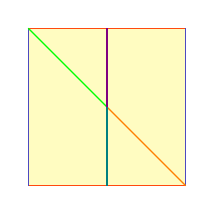
\begin{tikzpicture}

\draw[red, very thin] (-1,0) -- (1, 0);
\draw[blue, very thin] (-1,0) -- (-1, 2);
\draw[red, very thin] (-1,2) -- (1, 2);
\draw[blue, very thin] (1,0) -- (1, 2);


\fill[fill=yellow!80!white, fill opacity=0.3] (-1,0) rectangle (1,2);
\draw[green] (-1,2) -- (0,1);
\draw[orange] (0,1) -- (1,0);
\draw[teal] (0,0) -- (0,1);
\draw[violet] (0,1) -- (0,2);


\end{tikzpicture}
\hspace{50pt}
\begin{tikzpicture}

\node (K) at (.5,-2,0) [minimum width=100pt,minimum height=20pt,thick] {$K$};
\node (S) at (3,.5,0)  [minimum width=100pt,minimum height=20pt,thick] {$S^{1}$};
\coordinate (O) at (0,0,0);
\coordinate (A) at (0,\Width,0);
\coordinate (B) at (0,\Width,\Height);
\coordinate (C) at (0,0,\Height);
\coordinate (D) at (\Depth,0,0);
\coordinate (E) at (\Depth,\Width,0);
\coordinate (F) at (\Depth,\Width,\Height);
\coordinate (G) at (\Depth,0,\Height);



\coordinate (W) at (0,\Width/2,0);
\coordinate(X) at (\Depth,\Width/2,0);
\coordinate (Y) at (0,\Width/2,\Height);
\coordinate(Z) at (\Depth,\Width/2,\Height);




\draw[black] (C) -- (G); %Bottom Front
\draw[black] (B) -- (F); % Top Front
\draw[black] (C) -- (B); %Front Left
\draw[black] (G) -- (F); %Front Right

\draw[red] (C) -- (Z);
\draw[red] (Y) -- (F);


%% Following is for debugging purposes so you can see where the points are
%% These are last so that they show up on top
%\foreach \xy in {O, A, B, C, D, E, F, G, W, X, Y, Z}{
   % \node at (\xy) {\xy};
%}

\end{tikzpicture}

%%This is annoyingly off (3, 2)-cable
\hspace{50pt}
\begin{tikzpicture}

\node (K) at (.5,-2,0) [minimum width=100pt,minimum height=20pt,thick] {$K$};
\node (S) at (3,.5,0)  [minimum width=100pt,minimum height=20pt,thick] {$S^{1}$};

\coordinate (B) at (0,\Width,\Height);
\coordinate (C) at (0,0,\Height);

\coordinate (E) at (\Depth,\Width,0);
\coordinate (F) at (\Depth,\Width,\Height);
\coordinate (G) at (\Depth,0,\Height);





\coordinate (Y) at (0,\Width/3,\Height);
\coordinate (V) at (0,2*\Width/3,\Height);
\coordinate (L) at (\Height,\Width/3,\Height);
\coordinate (M) at (\Height,2*\Width/3,\Height);

\coordinate (W) at (2*\Depth/3,0,\Height);
\coordinate(Z) at (2*\Depth/3,\Width,\Height);
\coordinate (R) at (\Depth/3,0,\Height);
\coordinate (Q) at (\Depth/3,\Width,\Height);






\draw[black] (C) -- (G); %Bottom Front
\draw[black] (B) -- (F); % Top Front
\draw[black] (C) -- (B); %Front Left
\draw[black] (G) -- (F); %Front Right

\draw[red] (C) -- (Z);
\draw[red] (W) -- (M);
\draw[red] (V) -- (Q);
\draw[red] (R) -- (F);



%% Following is for debugging purposes so you can see where the points are
%% These are last so that they show up on top
\foreach \xy in {B, C, F, G, Y, Z, W, R, V, Q, L, M}{
    \node at (\xy) {\xy};
}

\end{tikzpicture}

\newpage
%%%%
\begin{tikzpicture}
\coordinate (O) at (0,0,0);
\coordinate (A) at (0,\Width,0);
\coordinate (B) at (0,\Width,\Height);
\coordinate (C) at (0,0,\Height);
\coordinate (D) at (\Depth,0,0);
\coordinate (E) at (\Depth,\Width,0);
\coordinate (F) at (\Depth,\Width,\Height);
\coordinate (G) at (\Depth,0,\Height);



\coordinate (W) at (0,\Width/2,0);
\coordinate(X) at (\Depth,\Width/2,0);
\coordinate (Y) at (0,\Width/2,\Height);
\coordinate(Z) at (\Depth,\Width/2,\Height);

\coordinate (a) at (4/3, 0, 0);
\coordinate(b) at (8/3, 0, 0);
\coordinate (c) at (4/3, 4, 0);
\coordinate(d) at (8/3, 4, 0);
\coordinate(e) at (4/3, 0,4);
\coordinate(f) at (8/3, 0, 4);
\coordinate(g) at (4/3, 4,4);
\coordinate(h) at (8/3, 4, 4);

%\draw[fill=magenta!80,fill opacity=0.3] (a) -- (b) -- (d) -- (e) -- cycle;
%\draw[fill=yellow!80,fill opacity=0.3] (C) -- (Z) -- (X) -- (O) -- cycle;
%\draw[fill=yellow!80,fill opacity=0.3] (Y) -- (F) -- (E) -- (W) -- cycle;

%\draw[magenta,thick] (a) -- (c);
%\draw[magenta,thick] (f) -- (d);

\draw[black] (e) -- (a);
\draw[black] (f) -- (b);

\draw[black] (g) -- (c);
\draw[black] (e) -- (g);
\draw[black] (a) -- (c);
\draw[black] (f) -- (g);
\draw[black] (f) -- (F);
\draw[black] (b) -- (c);
\draw[black] (b) -- (E);


\draw[black] (C) -- (G); %Bottom Back
\draw[black] (O) -- (D); %Bottom Front
\draw[black] (B) -- (F); % Top Front
\draw[black] (A) -- (E); %Top Back

\draw[black] (C) -- (O); %Bottom Left
\draw[black] (G) -- (D); %Bottom Right
\draw[black] (B) -- (A); %Top Left
\draw[black] (F) -- (E); %Top Right

\draw[black] (C) -- (B); %Front Left
\draw[black] (O) -- (A); %Back Left
\draw[black] (G) -- (F); %Front Right
\draw[black] (D) -- (E); %Back Right

%% Following is for debugging purposes so you can see where the points are
%% These are last so that they show up on top
%\foreach \xy in {O, A, B, C, D, E, F, G, W, X, Y, Z, a, b, c, d, e, f, g, h}{
   %\node at (\xy) {\xy};
%}

\end{tikzpicture}




\end{document}